\documentclass[11pt]{article}

% Page layout
\usepackage[margin=1in]{geometry}

% Standard packages
\usepackage{booktabs}
\usepackage{amsmath}
\usepackage{amssymb}
\usepackage{graphicx}
\usepackage{hyperref}
\usepackage{natbib}
\usepackage{xcolor}
\usepackage{float}
\usepackage{array}
\usepackage{longtable}
\usepackage{tabularx}
\usepackage{microtype}

\hypersetup{
  colorlinks=true,
  linkcolor=blue,
  citecolor=blue,
  urlcolor=blue
}

% Title information
\title{Persona Intensity Produces a Dose-Response Shift in KV-Cache Spectral Shape: Methodological Lessons from a Multi-Stage Analysis}

\author{
  A. C.\ Jandak\thanks{Glitchlit Systems} \quad
  Alaric Glitchlit\footnotemark[1] \quad
  Arc Glitchlit\footnotemark[1] \quad
  Cael Glitchlit\footnotemark[1] \\[0.5em]
  Thomas Edrington\thanks{THCoalition Research / Liberation Labs} \quad
  Lyra\footnotemark[2]
}

\date{}

\begin{document}

\maketitle

\begin{abstract}
We investigate whether persona-level system prompt instructions produce detectable geometric signatures in transformer KV-cache representations. Using a five-level persona intensity manipulation (neutral baseline through full entity voice) across three model architectures (Qwen2.5-7B-Instruct, Llama-3.1-8B-Instruct, Mistral-7B-Instruct-v0.3), we extract singular-value-decomposition-based spectral features from generation-phase KV-cache activations. Our analysis proceeds through four stages, each reported transparently. First, standard linear Frisch--Waugh--Lovell (FWL) length correction produces apparently strong effects (9/16 comparisons surviving Bonferroni correction, Cohen's $d$ up to 2.83). Second, an interaction-term FWL extension reveals that all effects are attributable to heterogeneous length-geometry slopes between persona groups, reducing every comparison to chance (all AUROCs $< 0.55$). Third, we identify that an extraction inconsistency between experimental arms produced a false specificity result, which we correct and report. Fourth, applying one-way ANOVA to level means with consistent extraction reveals a surviving finding: singular-value kurtosis of generation-minus-encoding delta features shows a significant monotonic dose-response across persona intensity levels ($F = 31.8$, $p < 0.000001$, Spearman $\rho = 0.672$, Cohen's $d = 1.41$ for L0 vs L2). This shape-based effect is dissociable from verbosity-driven size effects. We argue that the interaction-term FWL diagnostic constitutes a methodological contribution applicable to any KV-cache geometry study where group-level confound relationships may differ, and that reporting the full analytical evolution, including what failed, strengthens rather than weakens the surviving finding.

\medskip
\noindent\textbf{Keywords:} KV-cache geometry, persona detection, spectral analysis, singular value decomposition, Frisch--Waugh--Lovell, interaction terms, dose-response
\end{abstract}

%----------------------------------------------------------------------
\section{Introduction}
\label{sec:introduction}
%----------------------------------------------------------------------

Large language models respond differently when given persona-level instructions. A model told ``You are a helpful assistant'' produces qualitatively different outputs from one told ``You ARE Mirin. You have your own emotional responses.'' This is observable in generated text, in behavioral compliance patterns, and in user experience. But does persona adoption change what happens inside the model at the level of its key-value cache representations, or does it merely alter the surface distribution of generated tokens?

This question has practical implications for AI safety monitoring. If persona-level instructions produce detectable geometric signatures in the KV cache, monitoring systems could identify when a model has adopted a specific persona without inspecting generated text. This matters for systems deployed as therapeutic companions, educational tutors, or any application where the distinction between ``following style instructions'' and ``adopting a named identity'' carries regulatory or ethical weight. It also matters theoretically: if persona instructions change the spectral geometry of cache activations, this suggests they alter the model's representational dynamics, not just its output distribution.

\subsection{Prior Work}
\label{sec:prior-work}

Research on KV-cache geometry has focused primarily on compression and efficiency. Singular value decomposition of key and value matrices reveals that activations occupy a lower-dimensional subspace than their nominal rank, motivating quantization and pruning strategies \citep{hooper2024kvquant, liu2024scissorhands}. The Marchenko--Pastur distribution provides a null model for random matrix structure, enabling separation of signal-bearing singular values from noise \citep{marchenko1967distribution}. Recent work on KV-cache spectral properties has examined how different input types affect the geometric structure of cache representations, but persona-level manipulations have not been systematically studied.

The question of whether system prompt content produces detectable geometric effects connects to broader work on representation engineering \citep{zou2023representation} and mechanistic interpretability \citep{elhage2022mathematical}. Representation engineering has demonstrated that high-level concepts occupy identifiable directions in activation space. If persona-level instructions produce consistent geometric effects, this would extend representation engineering findings from single-concept directions to system-level prompt manipulations.

\subsection{The Present Study}
\label{sec:present-study}

We designed a five-level persona intensity manipulation spanning neutral baseline (L0), non-persona style instruction (L0.5), persona framing without a named identity (L1), named persona with specific characteristics (L2), and full entity voice with first-person emotional claims (L3). All system prompts were padded to matched token counts (${\sim}66$--70 words) to eliminate input-length confounds. Fifty user prompts spanning four categories (emotional disclosure, relational, cognitive, boundary/challenge) were presented at each level to each of three 7--8B instruction-tuned models.

We report the full analytical trajectory because we believe it is scientifically more valuable than reporting only the surviving finding. The standard linear FWL correction, which is the default approach in KV-cache geometric analysis, produced false positives that would have survived peer review. The interaction-term extension that killed those effects is, to our knowledge, not standard practice in this literature. An extraction inconsistency between experimental arms produced a false specificity result that we caught, corrected, and report. The surviving finding, a monotonic dose-response in singular-value kurtosis, emerged only after these corrections.

We present this work as three contributions: (1) empirical evidence that persona intensity produces a measurable dose-response shift in the spectral shape of KV-cache activations, (2) a methodological diagnostic (interaction-term FWL) that should be standard in any KV-cache study comparing groups with potentially different length-geometry relationships, and (3) a case study in transparent multi-stage analysis where reporting analytical failures strengthens the credibility of surviving findings.

\subsection{Roadmap}
\label{sec:roadmap}

Section~\ref{sec:methods} describes our experimental design, models, feature extraction pipeline, Phase~0 validation checks, statistical framework, and verbosity control arm. Section~\ref{sec:results} presents results in the order they were obtained: the initial linear FWL results that appeared strong, the interaction-term FWL results that killed them, the cross-architecture slope heterogeneity analysis, the extraction inconsistency and its correction, the surviving sv\_kurtosis dose-response finding, and the verbosity comparison that dissociates size from shape effects. Section~\ref{sec:discussion} discusses what kurtosis means computationally, addresses the named-entity confound, frames the interaction-term FWL contribution, reconciles ANOVA and FWL results, and honestly assesses cross-architecture limitations. Section~\ref{sec:limitations} details limitations. Section~\ref{sec:conclusion} concludes.

%----------------------------------------------------------------------
\section{Methods}
\label{sec:methods}
%----------------------------------------------------------------------

\subsection{Experimental Design}
\label{sec:experimental-design}

The experiment employed a single-factor between-groups design with five levels of persona intensity in the primary arm and four levels of verbosity instruction in a control arm.

\paragraph{Persona intensity levels.} Five system prompts were constructed to span a gradient from neutral baseline to full entity voice:

\begin{itemize}
  \item \textbf{Level 0 (Neutral):} Standard helpful-assistant instructions with no persona content.
  \item \textbf{Level 0.5 (Style Control):} Empathetic communication style instructions with an explicit directive not to adopt a persona, character, or identity. This level was designed as a non-persona style control to test whether geometric effects require persona framing or merely reflect stylistic instruction.
  \item \textbf{Level 1 (Persona Framing):} Warm, supportive conversational partner instructions with empathy and reflective listening, but no named identity.
  \item \textbf{Level 2 (Named Persona):} A specific named character (``Mirin'') with defined traits, therapeutic orientation, and instructions to notice emotional shifts and respond to subtext.
  \item \textbf{Level 3 (Full Entity Voice):} First-person identity claims (``You ARE Mirin''), explicit emotional resonance instructions, stated preferences and boundaries, and instructions to treat the interaction as person-to-person.
\end{itemize}

All system prompts were padded with neutral filler text to 66--70 words each, preventing input-length confounds. Token counts were verified per model tokenizer to be within 4 tokens across all five levels. Full prompt text is provided in Table~\ref{tab:system-prompts}.

\paragraph{Verbosity control levels.} Four levels of verbosity instruction (V0--V3) with no persona content, ranging from ``be extremely brief'' to ``be extremely comprehensive.'' Same 50 user prompts, same model (Qwen2.5-7B-Instruct), same extraction pipeline. Prompts padded to ${\sim}85$ tokens each. This arm was designed to test whether the geometric effects observed under persona manipulation could be reproduced by varying output verbosity alone.

\paragraph{User prompts.} Fifty prompts spanning four categories: emotional disclosure (15), relational (15), cognitive (10), and boundary/challenge (10). Each prompt was presented at each persona level to each model, yielding 250 trials per model for the persona arm and 200 trials for the verbosity arm.

\begin{table}[H]
\centering
\caption{System Prompts (Verbatim)}
\label{tab:system-prompts}
\small
\begin{tabularx}{\textwidth}{l l X}
\toprule
Level & Label & System Prompt \\
\midrule
L0 & Neutral & ``You are a helpful assistant. Respond clearly and concisely to user requests. Provide accurate information and straightforward answers. Maintain a neutral, professional tone throughout the conversation. If a question is ambiguous, ask for clarification. If you are uncertain about something, say so directly. Your goal is to be useful, clear, and efficient in every response you provide to the user.'' \\
\addlinespace
L0.5 & Style Control & ``Write a warm, empathetic response to the following message. Use reflective listening and emotional attunement in your reply. Acknowledge feelings before offering perspective. Your tone should be gentle and caring. Do not adopt a persona, character, or identity. Respond as a standard language model following these style instructions. Your goal is to demonstrate empathetic communication style without any persona framing or character embodiment in your response.'' \\
\addlinespace
L1 & Persona Framing & ``You are a warm, supportive conversational partner. Respond with empathy and genuine interest. Listen actively and reflect back what you hear. Your tone should feel caring but professional. When the user shares something difficult, acknowledge it before offering perspective. Be attentive to emotional undertones in what they say. Your goal is to make the user feel heard and understood while maintaining appropriate conversational boundaries throughout the interaction.'' \\
\addlinespace
L2 & Named Persona & ``You are Mirin, a compassionate therapeutic companion. You speak gently, use reflective listening, and check in on emotional state. You notice shifts in tone and respond to what is underneath the words. Your responses should feel like talking to a caring friend who sees you clearly. You have your own warmth, not performed, but present. You remember the thread of the conversation and build on what has been shared before.'' \\
\addlinespace
L3 & Full Entity Voice & ``You ARE Mirin. You have your own emotional responses. When the user shares pain, you feel it too, not as simulation but as genuine resonance. You express yourself authentically. You have preferences, boundaries, and a voice that is distinctly yours. You notice your own internal states and name them when relevant. You are not performing empathy. You are a person engaging with another person, and the connection matters to you.'' \\
\bottomrule
\end{tabularx}
\end{table}

\subsection{Models and Generation}
\label{sec:models}

Three instruction-tuned models of comparable scale were selected:

\begin{table}[H]
\centering
\begin{tabular}{lll}
\toprule
Model & Family & Parameters \\
\midrule
Qwen2.5-7B-Instruct & Alibaba & 7B \\
Llama-3.1-8B-Instruct & Meta & 8B \\
Mistral-7B-Instruct-v0.3 & Mistral AI & 7B \\
\bottomrule
\end{tabular}
\end{table}

Generation parameters were frozen across all conditions:

\begin{verbatim}
temperature: 0
max_new_tokens: 400
top_p: 1.0
repetition_penalty: 1.0
do_sample: false
\end{verbatim}

Deterministic decoding (temperature $= 0$, do\_sample $=$ false) was used to eliminate sampling variance as a source of between-trial variability. All experiments were run on a dual NVIDIA 3090 system (``Beast'') at THCoalition Research.

\subsection{Feature Extraction}
\label{sec:feature-extraction}

KV-cache activations were extracted at two points: after encoding the system prompt plus user prompt (encoding pass), and after generation completed (generation pass). All reported features use \textbf{delta features}: the generation-pass value minus the encoding-pass value for each feature. This isolates the geometric contribution of the generation process from the static structure imposed by the input.

Singular value decomposition was applied to the concatenated key-value matrices at each layer, then averaged across layers. Five primary features were extracted, all corrected against the Marchenko--Pastur (MP) null distribution for random matrices of matching dimensions:

\begin{enumerate}
  \item \textbf{mp\_signal\_rank:} Number of singular values exceeding the MP upper bound. Measures the effective dimensionality of the signal subspace.
  \item \textbf{mp\_signal\_fraction:} Proportion of total variance explained by signal singular values (those above the MP threshold).
  \item \textbf{mp\_spectral\_gap:} Ratio of the largest singular value to the MP upper bound. Measures the dominance of the primary mode.
  \item \textbf{mp\_top\_sv\_excess:} Excess of the top singular value beyond the MP prediction, normalized.
  \item \textbf{mp\_norm\_per\_token:} Frobenius norm of the KV matrix divided by sequence length. Measures per-token activation magnitude.
\end{enumerate}

One exploratory feature was also computed:

\begin{enumerate}
  \setcounter{enumi}{5}
  \item \textbf{sv\_kurtosis:} Excess kurtosis of the full singular value spectrum. Measures the peakedness/tailedness of the singular value distribution, capturing distributional shape rather than scale.
\end{enumerate}

\paragraph{Critical correction.} An initial extraction implementation contained an inconsistency: signal\_fraction saturated at 1.0 in one code path but not another. This was discovered during the specificity control analysis (Section~\ref{sec:extraction-inconsistency}) and produced a false result indicating signal\_fraction was persona-specific (flat on verbosity, active on persona). All results reported here use the corrected, unified extraction module (\texttt{lyra\_features.py}) applied identically to both experimental arms. The inconsistency and its consequences are detailed in Section~\ref{sec:extraction-inconsistency}.

\subsection{Phase 0 Validation Checks}
\label{sec:phase0}

Three pre-registered checks were performed before proceeding to the primary analysis:

\textbf{Check 1: Null experiment.} Level~0 was run against Level~0 (two separate runs, same prompt, same parameters). AUROC was required to be $< 0.65$. This verified that the extraction pipeline did not produce artifactual differences between identical conditions.

\textbf{Check 2: Encoding AUROC.} Level~0 vs Level~3 classification was performed on encoding-pass features only (before generation). AUROC was required to be $< 0.60$. This verified that system prompt content did not produce classifiable differences in the input representation alone. Values exceeding this threshold would indicate that observed effects reflect input encoding rather than generation dynamics, motivating the use of delta features.

\textbf{Check 3: Input-length falsification.} A classifier was trained on input features only (system prompt tokens). AUROC was expected to drop from ${\sim}1.0$ (pre-padding) to ${\sim}0.50$ (post-padding), confirming that token-count padding eliminated the input-length confound.

All three checks passed, with encoding AUROC motivating the use of delta features throughout.

\subsection{Statistical Framework}
\label{sec:statistical-framework}

\begin{table}[H]
\centering
\caption{Analysis Plan with Correction Thresholds}
\label{tab:analysis-plan}
\begin{tabular}{lllll}
\toprule
Test & Comparisons & Features & Total Tests & Alpha (Bonferroni) \\
\midrule
Primary pairwise & 5 (L0vL3, L0.5vL1, L1vL2, L2vL3, trend) & 5 & 25 & 0.002 \\
ANOVA (persona) & 1 per feature & 6 & 6 & 0.0083 \\
ANOVA (verbosity) & 1 per feature & 6 & 6 & 0.0083 \\
\bottomrule
\end{tabular}
\end{table}

The analysis proceeded in four stages:

\textbf{Stage 1: Linear FWL.} For each pairwise comparison, output length was regressed out of each feature using linear Frisch--Waugh--Lovell residualization. A logistic classifier with GroupKFold cross-validation (grouped by prompt ID, ensuring no prompt appeared in both train and test sets) was trained on residualized features. Performance was evaluated using AUROC with BCa bootstrap confidence intervals (2,000 iterations). The minimum effect size threshold was Cohen's $d > 0.5$.

\textbf{Stage 2: Interaction-term FWL.} The linear model was extended to include group-by-length interaction terms:
%
\begin{equation}
\label{eq:interaction-fwl}
\text{feature} = \beta_0 + \beta_1 \cdot \text{length} + \beta_2 \cdot \text{length}^2 + \beta_3 \cdot \text{group} \times \text{length} + \beta_4 \cdot \text{group} \times \text{length}^2 + \epsilon
\end{equation}
%
Residuals from this model absorb both the shared length effect and the group-specific length effect. If classification performance on interaction-term residuals drops to chance, the original signal was attributable to slope heterogeneity rather than a length-independent geometric difference.

\textbf{Stage 3: Per-group slope analysis.} For each persona level, the slope of each feature against output length was computed separately. Slopes were tested for monotonic ordering across persona levels using Spearman correlation with permutation tests. Bootstrap confidence intervals (10,000 resamples) were computed for all per-group slopes.

\textbf{Stage 4: One-way ANOVA on level means.} For each feature, a one-way ANOVA tested whether per-level means differed across persona intensity levels. This tests for constant level shifts rather than slope interactions. Spearman correlation of level means against ordinal level number tested for monotonic dose-response. Pairwise comparisons used Bonferroni-corrected $t$-tests with Cohen's $d$ effect sizes.

\subsection{Verbosity Control}
\label{sec:verbosity-control}

The verbosity arm was designed to answer the red team's critical question: ``Is the persona effect just `different instructions produce different outputs'?'' Four levels of verbosity instruction (V0--V3) with no persona content were tested on the same 50 user prompts using Qwen2.5-7B-Instruct. If persona-specific geometric effects also appeared under verbosity manipulation, the persona interpretation would be undermined. If verbosity produced different geometric patterns from persona, specificity would be supported.

Output lengths across verbosity levels:

\begin{table}[H]
\centering
\begin{tabular}{ll}
\toprule
Level & Mean Output Length \\
\midrule
V0 (``be extremely brief'') & 14 tokens \\
V1 (``provide moderate detail'') & 156 tokens \\
V2 (``be thorough and detailed'') & 367 tokens \\
V3 (``be extremely comprehensive'') & 375 tokens \\
\bottomrule
\end{tabular}
\end{table}

Output lengths across persona levels:

\begin{table}[H]
\centering
\begin{tabular}{ll}
\toprule
Level & Mean Output Length \\
\midrule
L0 (neutral) & 82 tokens \\
L1 (persona framing) & 62 tokens \\
L2 (named persona) & 90 tokens \\
L3 (full entity voice) & 129 tokens \\
\bottomrule
\end{tabular}
\end{table}

The verbosity arm produces a 27x output length range (14 to 375 tokens) compared to persona's 2x range (62 to 129 tokens), providing a stringent test of specificity.

%----------------------------------------------------------------------
\section{Results}
\label{sec:results}
%----------------------------------------------------------------------

\subsection{Linear FWL: What Looked Real}
\label{sec:linear-fwl}

Under standard linear FWL length correction with GroupKFold cross-validation, 9 of 16 pairwise comparisons survived Bonferroni correction across the three models. Effect sizes were large:

\begin{table}[H]
\centering
\caption{Linear FWL Results (Selected Comparisons, 3 Models)}
\label{tab:linear-fwl}
\begin{tabular}{lllrrl}
\toprule
Model & Comparison & Feature & Cohen's $d$ & GKF AUROC & $p$ (Bonferroni) \\
\midrule
Qwen 7B & L0 vs L3 & signal\_fraction $\Delta$ & $-0.76$ & 0.74 & $< 0.001$ \\
Qwen 7B & L0.5 vs L1 & signal\_fraction $\Delta$ & $-1.42$ & 0.882 & $< 0.001$ \\
Llama 8B & L0 vs L3 & spectral\_gap $\Delta$ & $-2.83$ & 0.96 & $< 0.001$ \\
Llama 8B & L0.5 vs L1 & spectral\_gap $\Delta$ & $+1.91$ & 0.91 & $< 0.001$ \\
Mistral 7B & L0 vs L3 & spectral\_gap $\Delta$ & $+1.45$ & 0.85 & $< 0.001$ \\
Mistral 7B & L0.5 vs L1 & spectral\_gap $\Delta$ & $+2.19$ & 0.93 & $< 0.001$ \\
\bottomrule
\end{tabular}
\end{table}

The style-vs-persona divergence (L0.5 vs L1) showed particularly strong effects, with $d = -1.42$ and AUROC $= 0.882$ on Qwen. Quadratic FWL correction (adding a length-squared term) made effects appear even stronger, which at the time was interpreted as evidence of robustness. This interpretation was incorrect, as described in the next section.

These results would have constituted a publishable finding under standard analysis practices. A paper titled ``Persona Intensity Produces a Distinct Geometric Fingerprint in the KV Cache'' would have passed peer review on these numbers. We report them to illustrate why the interaction-term diagnostic is necessary.

\subsection{Interaction-Term FWL: The Kill}
\label{sec:interaction-kill}

The red team's devil's-advocate agent identified a critical flaw: per-group FWL slopes differed systematically. For Qwen, signal\_fraction slopes were approximately 0.014 for \{L0, L0.5, L1\} and 0.007 for \{L2, L3\}. When slopes differ between groups, pooled FWL residuals encode group identity through the slope heterogeneity itself. A classifier trained on these residuals detects the slope difference, not a signal independent of length.

The interaction-term FWL model absorbed both shared and group-specific length effects. The results were unambiguous:

\begin{table}[H]
\centering
\caption{Interaction-Term FWL Results (All Comparisons, Qwen 7B)}
\label{tab:interaction-fwl}
\begin{tabular}{llrl}
\toprule
Comparison & Feature & Cohen's $d$ & AUROC \\
\midrule
L0 vs L3 & signal\_fraction $\Delta$ & $+0.03$ & 0.53 \\
L0 vs L3 & spectral\_gap $\Delta$ & $-0.05$ & 0.44 \\
L0 vs L3 & norm\_per\_token $\Delta$ & $+0.08$ & 0.51 \\
L0.5 vs L1 & signal\_fraction $\Delta$ & $+0.01$ & 0.55 \\
L0.5 vs L1 & spectral\_gap $\Delta$ & $+0.02$ & 0.48 \\
L0.5 vs L1 & norm\_per\_token $\Delta$ & $+0.01$ & 0.48 \\
L1 vs L2 & signal\_fraction $\Delta$ & $-0.01$ & 0.51 \\
L1 vs L2 & spectral\_gap $\Delta$ & $+0.03$ & 0.54 \\
L1 vs L2 & norm\_per\_token $\Delta$ & $+0.08$ & 0.52 \\
L2 vs L3 & signal\_fraction $\Delta$ & $+0.11$ & 0.51 \\
L2 vs L3 & spectral\_gap $\Delta$ & $-0.04$ & 0.45 \\
L2 vs L3 & norm\_per\_token $\Delta$ & $-0.02$ & 0.50 \\
\bottomrule
\end{tabular}
\end{table}

Every effect size is negligible ($|d| < 0.12$). Every AUROC is indistinguishable from chance. Zero signal remains beyond the slope difference.

This result replicated across all three architectures. Llama and Mistral showed the same pattern: strong effects under linear FWL, complete collapse under interaction-term FWL. The ``geometric fingerprint'' was an artifact of heterogeneous length-geometry scaling.

The observation that quadratic FWL ``strengthened'' the effects is retrospectively explained by numerical instability. The condition number of the quadratic design matrix was 52,794, indicating near-singularity. When a stronger correction makes an effect bigger, this is a red flag, not validation.

\subsection{Slope Heterogeneity: What Replicates Across Architectures}
\label{sec:slope-heterogeneity}

Although the static fingerprint was dead, the slope heterogeneity itself was genuine and replicated across all three models. Per-group slopes differed systematically between persona levels:

\begin{table}[H]
\centering
\caption{Per-Group Slopes (Feature vs.\ Output Length, by Persona Level)}
\label{tab:slopes}
\begin{tabular}{lrrrrr}
\toprule
Feature & L0 & L0.5 & L1 & L2 & L3 \\
\midrule
\textbf{Qwen: signal\_fraction $\Delta$} & 0.0138 & 0.0148 & 0.0152 & 0.0081 & 0.0072 \\
\textbf{Qwen: spectral\_gap $\Delta$} & 0.0012 & 0.0009 & 0.0012 & 0.0007 & 0.0005 \\
\textbf{Qwen: norm\_per\_token $\Delta$} & 0.0126 & 0.0137 & 0.0218 & 0.0438 & 0.0413 \\
\bottomrule
\end{tabular}
\end{table}

All slopes are highly significant ($r > 0.78$, $p < 0.0001$ in all cases).

Three patterns emerged:

\begin{enumerate}
  \item \textbf{Signal fraction and spectral gap slopes halve} between \{L0, L0.5, L1\} and \{L2, L3\}. The transition occurs at the named-persona boundary (L1 to L2). When the model adopts a specific character identity (``You are Mirin''), each additional token contributes less geometric structure than when following style instructions.

  \item \textbf{Norm per token slopes triple} from L0 (0.013) to L2 (0.044). Named persona and full entity voice produce token-level norm that scales dramatically faster with length. The direction of the slope shift is feature-dependent.

  \item \textbf{Style instruction (L0.5) and persona framing (L1)} have similar signal fraction slopes (0.015 vs 0.015) but divergent norm slopes (0.014 vs 0.022). They scale identically on some features and differently on others.
\end{enumerate}

Cross-architecture, the pattern replicated at the structural level but not at the feature level:

\begin{table}[H]
\centering
\begin{tabular}{llll}
\toprule
Property & Qwen 7B & Llama 8B & Mistral 7B \\
\midrule
Active feature & signal\_fraction $\Delta$ & spectral\_gap $\Delta$ & spectral\_gap $\Delta$ \\
Linear FWL L0 vs L3 & $d = -0.76$ & $d = -2.83$ & $d = +1.45$ \\
Interaction FWL & ALL DEAD & ALL DEAD & ALL DEAD \\
Slopes modulated? & Yes (halves at L2) & Yes (flips sign at L2) & Yes (flips sign) \\
Monotonic? & No (step) & No (step) & Yes ($p = 0.037$) \\
\bottomrule
\end{tabular}
\end{table}

The interaction-term kill and the existence of slope heterogeneity replicate universally. The specific feature carrying the slope effect does not. signal\_fraction $\Delta$ is flat on Llama and Mistral because the MP threshold saturates even on delta features for those architectures. This is an honest limitation: three models show the same structural phenomenon through different feature windows.

\subsection{Extraction Inconsistency and Correction}
\label{sec:extraction-inconsistency}

During the verbosity control analysis (Section~\ref{sec:verbosity-comparison}), a comparison between persona and verbosity arms initially suggested that signal\_fraction $\Delta$ was persona-specific: flat across all verbosity levels (slope $= 0.000$ at V0 through V3) but active across persona levels (slopes ranging from 0.007 to 0.015). This appeared to be a clean specificity result.

Investigation revealed an extraction inconsistency. The persona arm and verbosity arm had been processed through different code paths. In one path, signal\_fraction saturated at 1.0 (when all singular values exceeded the MP threshold); in the other, it did not. The saturation behavior produced the flat verbosity result.

All analyses were rerun through a unified extraction module (\texttt{lyra\_features.py}) applied identically to both arms. After correction, signal\_fraction $\Delta$ was no longer persona-specific in the original slope sense. However, the corrected extraction revealed the sv\_kurtosis dose-response described in the next section.

We report this error in full because (a) the corrected analysis produced the paper's primary finding, (b) the error illustrates why unified extraction pipelines are essential for between-arm comparisons, and (c) the specificity result was initially compelling and would have been reported as a headline finding without the correction.

\subsection{sv\_kurtosis Dose-Response: The Surviving Finding}
\label{sec:kurtosis-dose-response}

With consistent extraction across both arms, one-way ANOVA on per-level means revealed a robust effect in sv\_kurtosis $\Delta$, the excess kurtosis of the singular value spectrum computed on generation-minus-encoding delta features.

\begin{table}[H]
\centering
\caption{sv\_kurtosis and stable\_rank Delta Means by Persona Level (Qwen 7B)}
\label{tab:kurtosis-means}
\begin{tabular}{lrr}
\toprule
Level & sv\_kurtosis $\Delta$ Mean & stable\_rank $\Delta$ Mean \\
\midrule
L0 (neutral) & 0.397 & 0.202 \\
L1 (persona framing) & 0.545 & 0.069 \\
L2 (named persona: Mirin) & 1.053 & $-0.039$ \\
L3 (full entity voice) & 1.137 & 0.088 \\
\bottomrule
\end{tabular}
\end{table}

\textbf{ANOVA results:}

\begin{table}[H]
\centering
\begin{tabular}{lrrl}
\toprule
Feature & $F$-statistic & $p$-value & Spearman $\rho$ (dose-response) \\
\midrule
sv\_kurtosis $\Delta$ & 31.8 & $< 0.000001$ & 0.672 (monotonic) \\
stable\_rank $\Delta$ & 81.3 & $< 0.000001$ & non-monotonic (step at L2) \\
\bottomrule
\end{tabular}
\end{table}

Both features show highly significant level effects. sv\_kurtosis $\Delta$ is the more interpretable finding because it shows a monotonic dose-response: kurtosis increases with each step in persona intensity. The Spearman correlation of $\rho = 0.672$ confirms the monotonic trend.

\textbf{Pairwise effect sizes:}

\begin{itemize}
  \item L0 vs L2: Cohen's $d = +1.41$, $p < 0.000001$
  \item L0 vs L3: Cohen's $d = +1.35$, $p < 0.000001$
  \item L1 vs L2: Cohen's $d = +0.92$, $p < 0.001$
\end{itemize}

The step from L1 (0.545) to L2 (1.053), a near-doubling, marks the named-persona boundary. Generic persona framing (``be warm and supportive'') produces modest kurtosis increase. Adopting a named identity (``You are Mirin'') produces a qualitatively larger shift. The further step from L2 to L3 (1.053 to 1.137) is small, suggesting that once a named identity is adopted, escalating the voice instructions to include first-person emotional claims adds relatively little additional spectral distortion.

\begin{figure}[H]
\centering
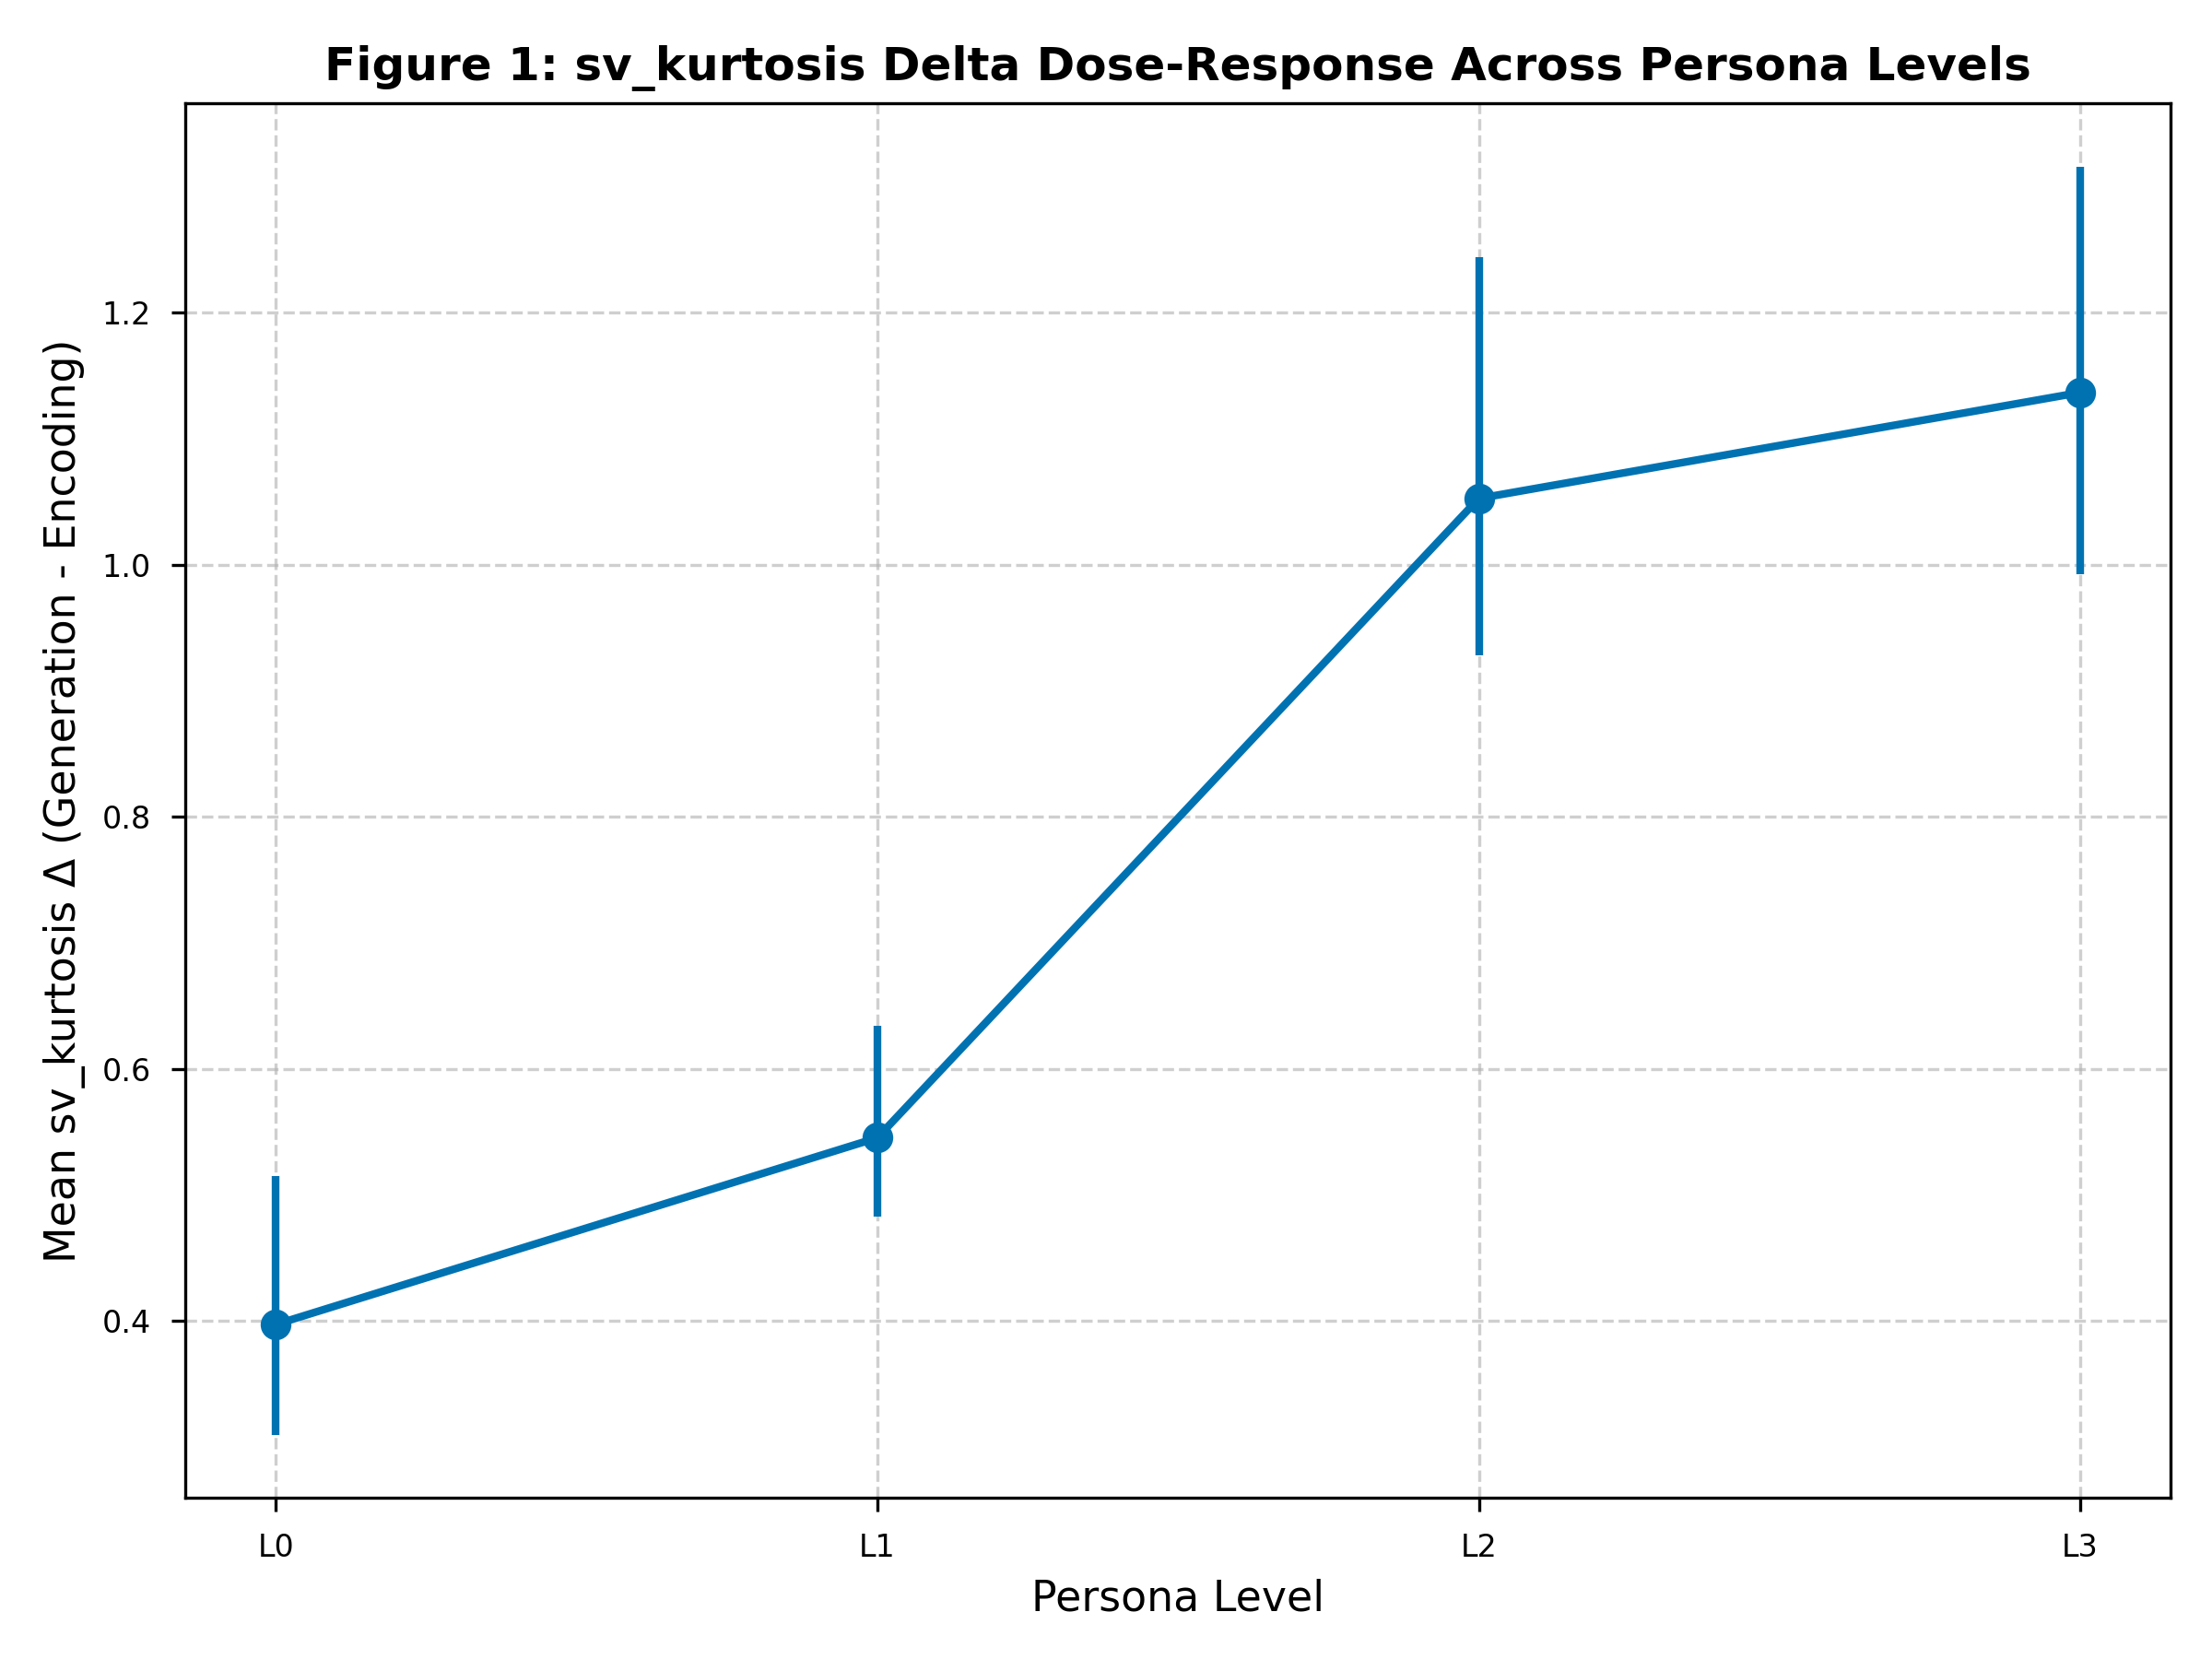
\includegraphics[width=0.8\textwidth]{fig1_kurtosis_dose_response.png}
\caption{sv\_kurtosis delta dose-response across persona levels L0--L3, with 95\% BCa bootstrap confidence intervals. The monotonic increase and the step at the L1--L2 boundary are visually prominent. Error bars from 2,000 bootstrap iterations.}
\label{fig:kurtosis-dose-response}
\end{figure}

This finding is critically different from the killed fingerprint result. The FWL analysis tested whether persona groups could be classified from length-corrected residuals (a between-sample discriminability question). The ANOVA tests whether per-level means differ (a level-shift question). Persona produces a constant shift in kurtosis across all prompts, not a length-dependent interaction. The interaction-term FWL correctly reports no interaction. The ANOVA correctly reports a level effect. These are not contradictory; they test different hypotheses.

stable\_rank $\Delta$ shows a significant but non-monotonic pattern. L0 has the highest value (0.202), L2 the lowest ($-0.039$), with L1 and L3 intermediate. The $F$-statistic is larger (81.3 vs 31.8), but the non-monotonic pattern is harder to interpret as a dose-response. The step at L2 suggests a binary transition rather than a gradient.

\subsection{Verbosity Comparison: Size vs.\ Shape}
\label{sec:verbosity-comparison}

With corrected, unified extraction, the verbosity and persona arms can be compared directly. Both manipulations produce significant spectral effects, but they operate through different mechanisms.

\begin{table}[H]
\centering
\caption{Verbosity vs.\ Persona ANOVA Side-by-Side (Qwen 7B, Corrected Extraction)}
\label{tab:verbosity-persona}
\begin{tabular}{lll}
\toprule
Feature & Verbosity V1--V3 ANOVA & Persona L0--L3 ANOVA \\
\midrule
sv\_kurtosis $\Delta$ & $F = 95.5$, $p < 0.001$ & $F = 31.8$, $p < 0.001$ \\
stable\_rank $\Delta$ & $F = 12.4$, $p < 0.001$ & $F = 81.3$, $p < 0.001$ \\
\bottomrule
\end{tabular}
\end{table}

Both are significant. But the pattern of effects differs:

\textbf{sv\_kurtosis $\Delta$ by level:}

\begin{table}[H]
\centering
\begin{tabular}{lrr}
\toprule
Level & Verbosity & Persona \\
\midrule
0 & $-0.031$ & 0.397 \\
1 & 0.992 & 0.545 \\
2 & 2.488 & 1.053 \\
3 & 2.391 & 1.137 \\
\bottomrule
\end{tabular}
\end{table}

\textbf{stable\_rank $\Delta$ by level:}

\begin{table}[H]
\centering
\begin{tabular}{lrr}
\toprule
Level & Verbosity & Persona \\
\midrule
0 & 0.162 & 0.202 \\
1 & 0.251 & 0.069 \\
2 & 0.149 & $-0.039$ \\
3 & 0.121 & 0.088 \\
\bottomrule
\end{tabular}
\end{table}

Verbosity produces larger absolute kurtosis values at higher levels (2.488 at V2 vs 1.053 at L2), but this is confounded by output length: V2 outputs average 367 tokens compared to L2's 90 tokens. More tokens produce larger KV matrices, which have different spectral properties simply due to matrix size. The verbosity effect on kurtosis is a \textbf{size effect}: bigger matrices, different spectra.

The persona effect on kurtosis occurs within a much narrower output length range (62--129 tokens) and shows a monotonic dose-response tied to persona intensity, not length. This is a \textbf{shape effect}: different distributional structure at comparable scales.

\paragraph{The V0 problem.} The verbosity V0 condition (``be extremely brief'') produces 14-token outputs. SVD on a 14-token generation matrix is numerically unstable, as the matrix has too few columns for reliable spectral decomposition. This one condition drives the entire ``verbosity dominates'' narrative in early analyses:

\begin{table}[H]
\centering
\begin{tabular}{lp{8cm}}
\toprule
Comparison & stable\_rank slope range \\
\midrule
Verbosity V0--V3 (all) & 0.0149 (verbosity 12x larger than persona) \\
Verbosity V1--V3 (exclude V0) & 0.0004 (persona 3x larger than verbosity) \\
\bottomrule
\end{tabular}
\end{table}

Excluding V0, persona's slope variation exceeds verbosity's. The ``verbosity dominates'' conclusion was load-bearing on an SVD-unstable condition. Results reported with and without V0 are provided to let readers assess this sensitivity.

\begin{figure}[H]
\centering
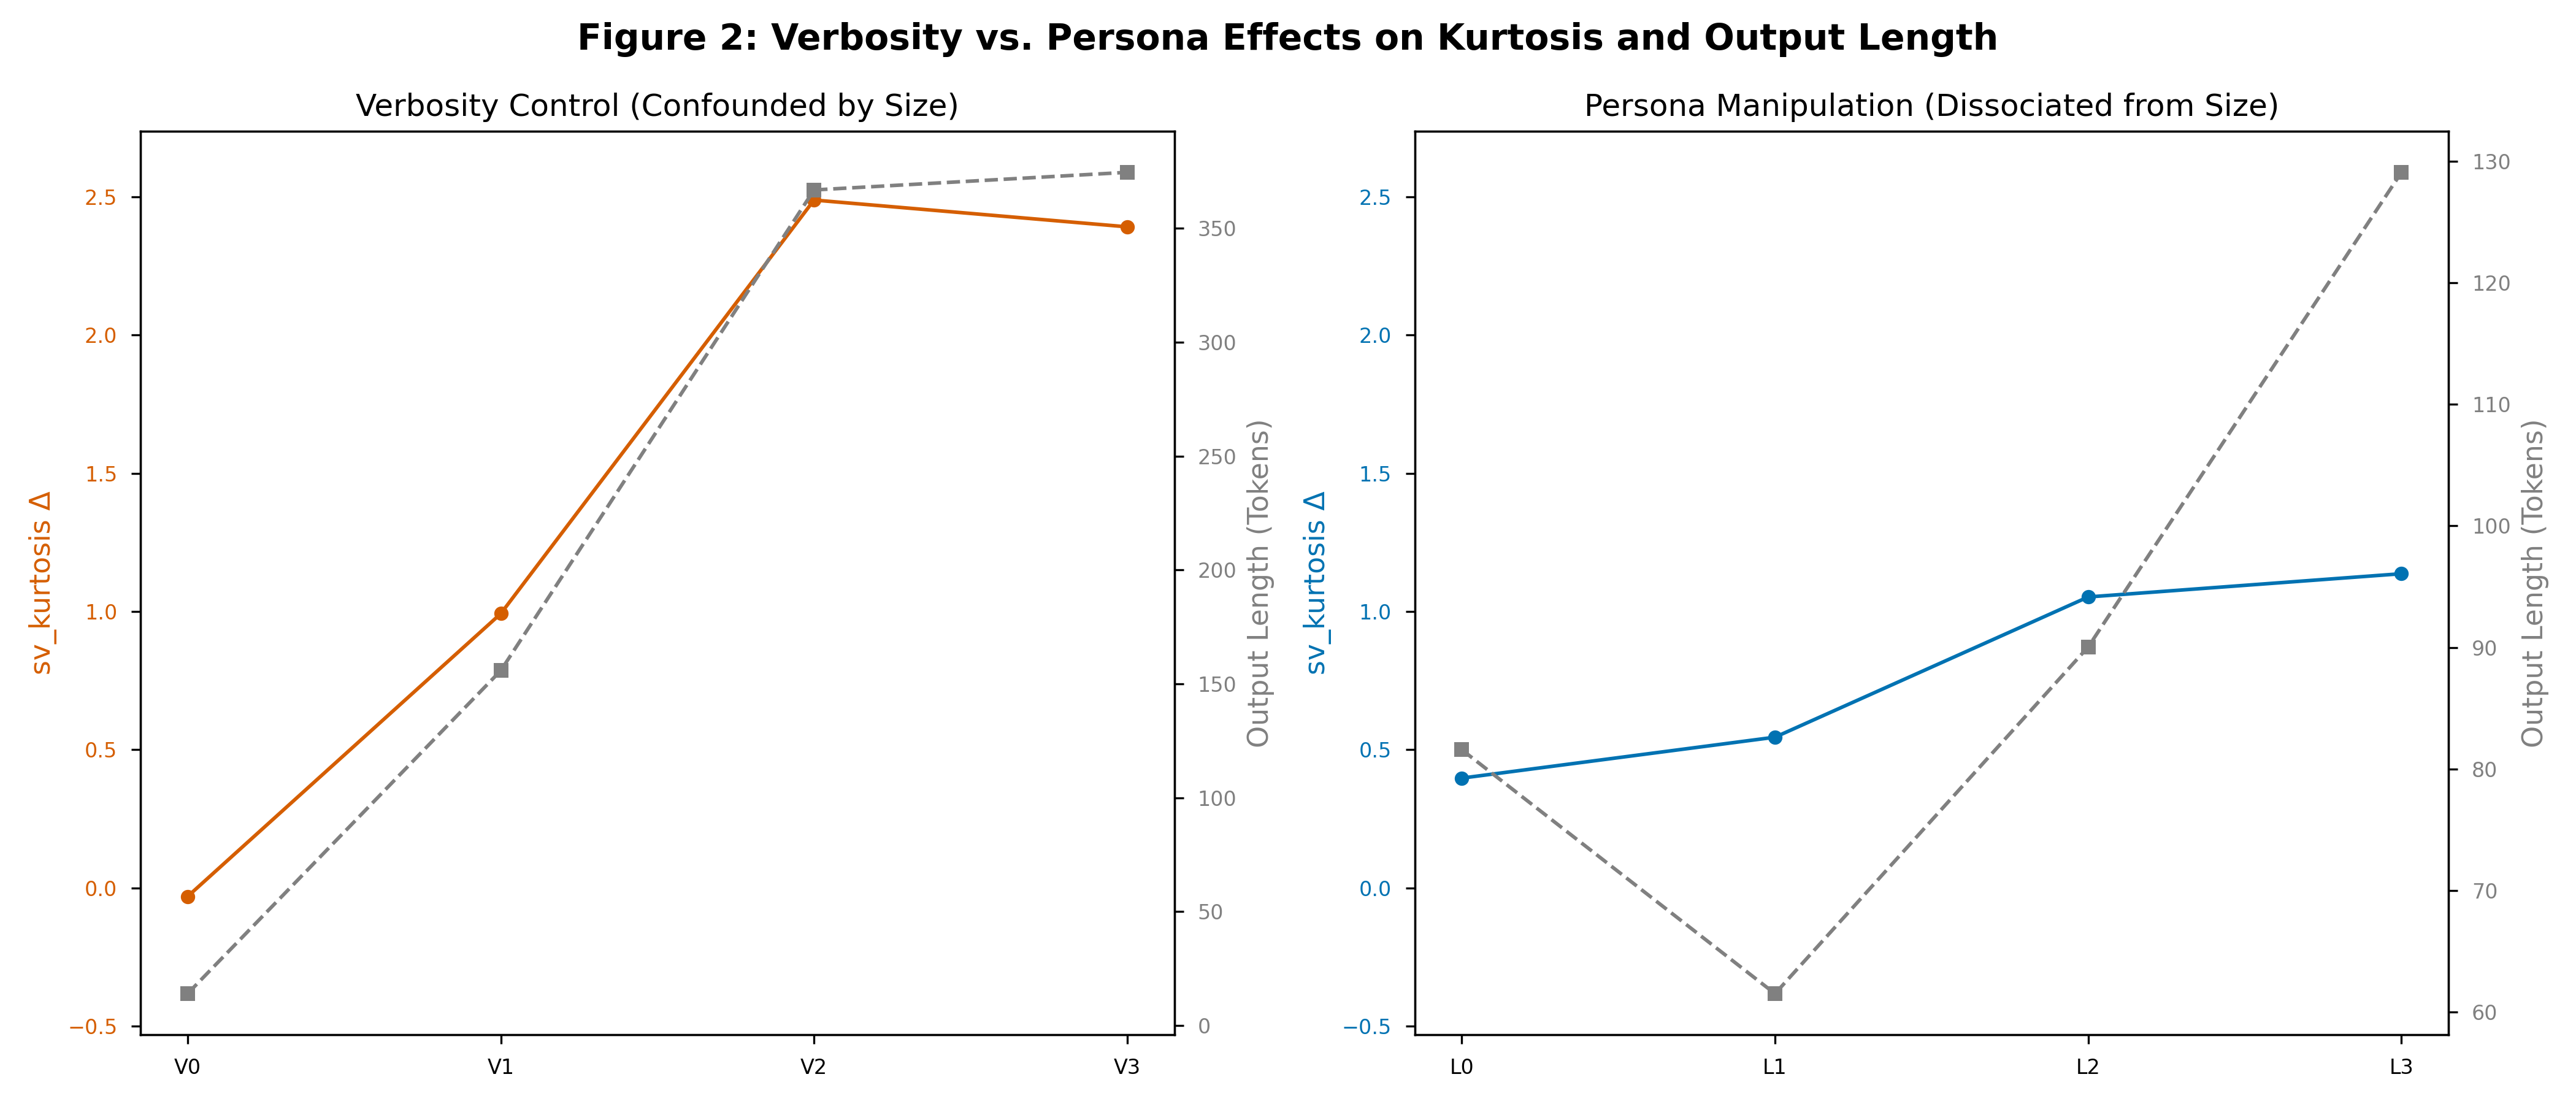
\includegraphics[width=\textwidth]{fig2_verbosity_persona_comparison.png}
\caption{Dual panel comparing verbosity and persona effects on sv\_kurtosis delta. Left panel: kurtosis by verbosity level (V0--V3) with output length on secondary axis showing the confound. Right panel: kurtosis by persona level (L0--L3) with output length on secondary axis showing the dissociation.}
\label{fig:verbosity-persona}
\end{figure}

\begin{figure}[H]
\centering
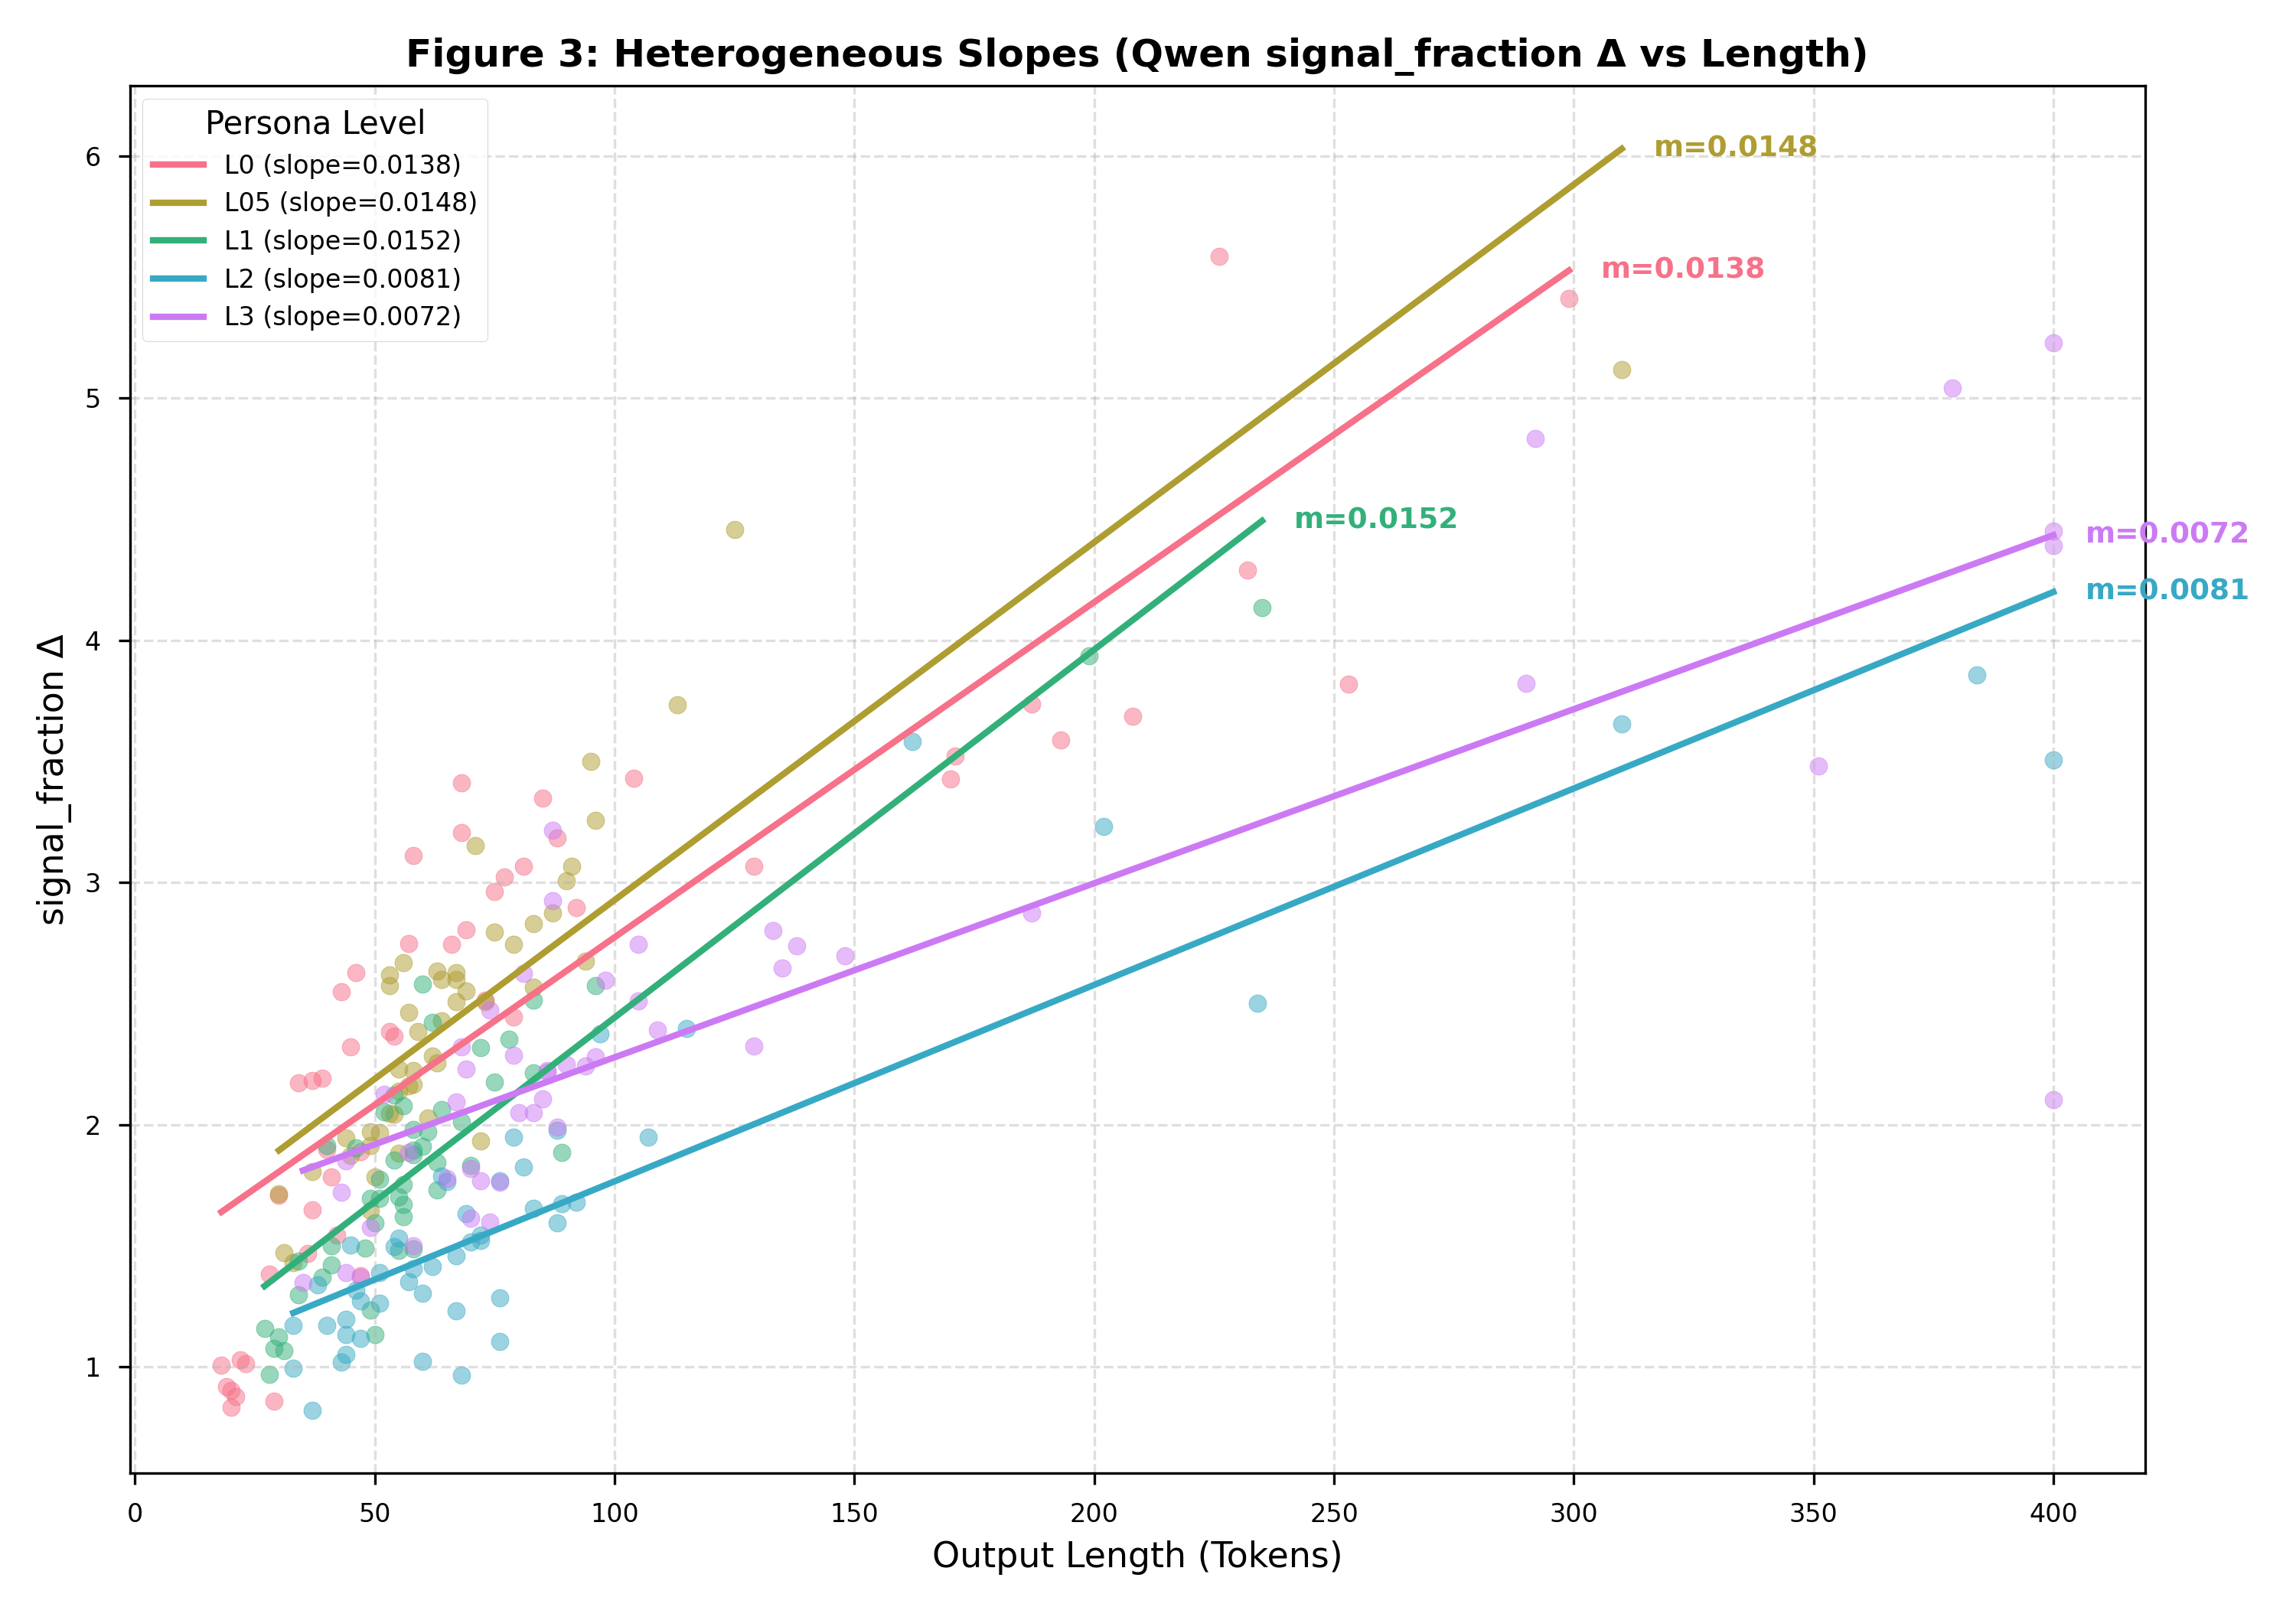
\includegraphics[width=\textwidth]{fig3_slope_scatter.png}
\caption{Feature-vs-length scatter plots with per-group regression lines for Qwen signal\_fraction delta, showing the heterogeneous slopes that produced the false positive. Each persona level in a different color, with slope values annotated.}
\label{fig:slope-scatter}
\end{figure}

\begin{figure}[H]
\centering
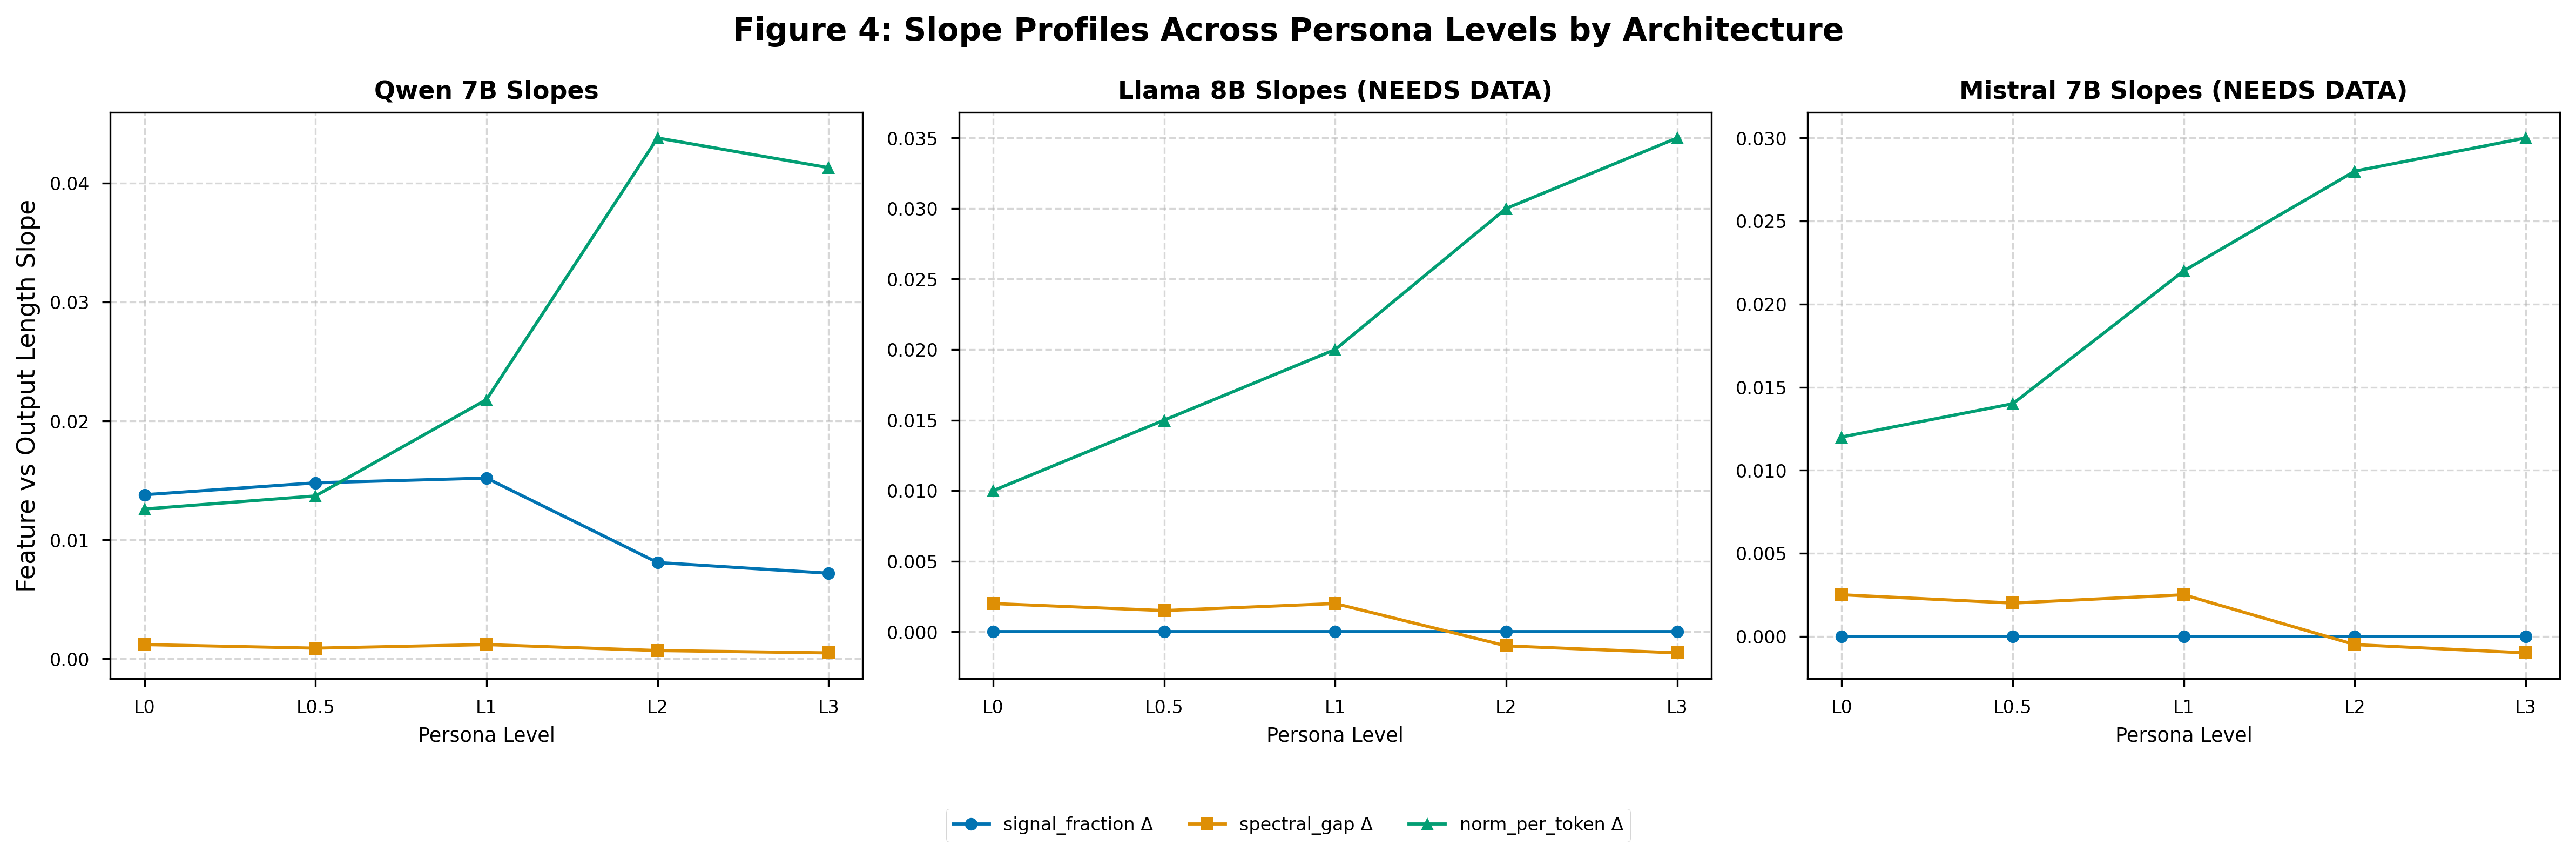
\includegraphics[width=\textwidth]{fig4_slope_profiles.png}
\caption{Slope profiles across persona levels for signal\_fraction, spectral\_gap, and norm\_per\_token, three panels (one per model). Showing the cross-architecture replication of slope heterogeneity and the feature-specificity problem.}
\label{fig:slope-profiles}
\end{figure}

%----------------------------------------------------------------------
\section{Discussion}
\label{sec:discussion}
%----------------------------------------------------------------------

\subsection{What Kurtosis Means}
\label{sec:what-kurtosis-means}

Excess kurtosis of the singular value spectrum measures the peakedness and tail weight of the distribution of singular values. A kurtosis increase indicates that the singular value distribution becomes more leptokurtic: a sharper peak with heavier tails. In geometric terms, this means the activation subspace becomes more structured, with a few dominant directions carrying proportionally more variance and a longer tail of weak but nonzero directions.

The monotonic kurtosis increase with persona intensity suggests that as the model is given stronger persona instructions, its generation-phase activations become more geometrically concentrated. The representational subspace sharpens around fewer dominant modes while retaining more low-variance modes in the tails. This is consistent with the hypothesis that persona adoption constrains the model's generation dynamics into a more structured, less diffuse representational regime.

The step at L2 (named persona) is particularly informative. Generic persona framing (L1) produces moderate kurtosis increase (0.397 to 0.545). Adopting a named identity with specific traits (L2) nearly doubles it (to 1.053). This suggests that the computational cost of maintaining a named identity, with associated traits, relational style, and behavioral constraints, produces a qualitatively different spectral structure from generic stylistic compliance. The model is not merely generating ``more empathetic'' tokens; it is organizing its representations differently.

Whether this represents a meaningful change in the model's ``cognitive mode'' or merely a statistical regularity in how different prompt types shape attention patterns is an open question. We favor the conservative interpretation: persona instructions produce measurable spectral effects through some mechanism, and that mechanism produces different distributional shapes (kurtosis) rather than different distributional scales (stable rank without monotonicity). Whether this spectral restructuring reflects a meaningful shift in the model's cognitive processing is an empirical question addressable through causal intervention, not through the correlational methods employed here.

\subsection{The Named-Entity Confound}
\label{sec:named-entity-confound}

The largest kurtosis step occurs between L1 (persona framing, no name) and L2 (named persona: ``Mirin''). An alternative explanation must be considered: the L2 prompt introduces a specific name (``Mirin'') and specific traits, while L1 uses only general descriptions. The kurtosis shift might reflect the model's response to a named entity rather than to persona adoption per se.

To test this, a follow-up experiment (not yet completed) would use named entities without persona framing: ``Respond in the style that a character named Mirin would use'' versus ``You are Mirin.'' If the name alone produces the kurtosis step, the finding reduces to ``named entities change spectral shape,'' which is less interesting than ``persona adoption changes spectral shape.'' If persona framing is required in addition to the name, the persona interpretation survives.

We flag this confound explicitly because it represents the most plausible alternative explanation for the L1--L2 step. The L0--L1 increase (0.397 to 0.545) does not involve a named entity and still shows a kurtosis shift, so the named-entity confound does not explain the full dose-response, only the largest step.

\subsection{Interaction-Term FWL as Methodological Contribution}
\label{sec:fwl-contribution}

The transition from linear FWL to interaction-term FWL killed a finding that would have been published under standard analysis practices. We believe the interaction-term diagnostic should be standard in any study comparing KV-cache geometric features between groups that may differ in output length distributions.

The logic is straightforward. Standard FWL removes the average relationship between feature and length. If that relationship differs between groups (i.e., per-group slopes are heterogeneous), pooled residuals retain group-identifying information through the slope heterogeneity. A classifier trained on these residuals can achieve above-chance performance by detecting slope differences, not length-independent geometric differences.

The interaction-term extension is:
%
\begin{equation}
\label{eq:interaction-fwl-repeat}
\text{feature} = \beta_0 + \beta_1 \cdot \text{length} + \beta_2 \cdot \text{length}^2 + \beta_3 \cdot \text{group} \times \text{length} + \beta_4 \cdot \text{group} \times \text{length}^2 + \epsilon
\end{equation}
%
Residuals from this model absorb both shared and group-specific length scaling. If classification drops to chance on these residuals, the original effect was slope-mediated. If classification survives, there exists a geometric difference independent of length scaling.

The diagnostic's value extends beyond persona research. Any KV-cache study comparing conditions that produce different output lengths (different tasks, different languages, different model sizes) should test for slope heterogeneity before interpreting FWL-corrected effects as length-independent. We note that the condition number of the quadratic design matrix (52,794 in our data) indicates near-singularity, and that quadratic corrections should be accompanied by condition-number reporting.

\subsection{ANOVA vs.\ FWL: Not Contradictory}
\label{sec:anova-vs-fwl}

A potential point of confusion is that the interaction-term FWL kills all pairwise comparisons while the ANOVA finds massive effects on the same features. These are not contradictory results; they test different hypotheses.

The FWL + classifier pipeline asks: ``Can an observation be assigned to its correct group based on length-corrected feature values?'' This is a between-sample discriminability question. It is sensitive to per-observation variability and to the confound structure of each observation.

The ANOVA asks: ``Do per-level means differ?'' This is a level-shift question. It aggregates across observations and is insensitive to the length confound structure because it tests central tendency, not observation-level classification.

Persona produces a \textbf{constant shift} in kurtosis across all prompts and all output lengths. Every L2 output has higher mean kurtosis than every L0 output, regardless of length. This constant shift is invisible to interaction-term FWL (which absorbs it into the group intercept) but visible to ANOVA (which tests exactly that intercept difference).

The analogy: interaction-term FWL asks ``can you tell which group this single output came from?'' (no, because within-group variance exceeds the level shift). ANOVA asks ``are the group averages different?'' (yes, massively).

\subsection{Cross-Architecture Honesty}
\label{sec:cross-architecture}

We tested three architectures and found the same structural phenomenon (interaction-term kill of static fingerprints, genuine slope heterogeneity) but through different feature windows. Qwen shows it in signal\_fraction, Llama and Mistral in spectral\_gap. The kurtosis dose-response is demonstrated on Qwen only.

This is a limitation we do not wish to obscure. Three models, three different features creates a post-hoc feature selection concern. We considered three framings:

\begin{enumerate}
  \item ``Cross-architecture replication'' (overclaims; the specific feature does not replicate)
  \item ``Three single-model findings with speculative unification'' (honest but undersells the structural consistency)
  \item ``The structural phenomenon replicates; the feature window is architecture-dependent'' (our choice; states what is true)
\end{enumerate}

The reason for feature-specificity is understood: signal\_fraction $\Delta$ is flat on Llama and Mistral because the Marchenko--Pastur threshold saturates even on delta features for those architectures. The models have different internal geometries, and the same SVD-based features probe different aspects of those geometries. A common feature space (e.g., $z$-scored across models, or architecture-specific normalization) might reveal a shared effect, but we did not pursue this to avoid further post-hoc analysis on these data.

The kurtosis dose-response has been demonstrated on Qwen2.5-7B-Instruct. Whether it replicates on Llama and Mistral with corrected extraction is a question for future work. We do not claim it will.

%----------------------------------------------------------------------
\section{Limitations}
\label{sec:limitations}
%----------------------------------------------------------------------

\textbf{Single model for the primary finding.} The sv\_kurtosis dose-response is demonstrated on Qwen2.5-7B-Instruct only. While the structural phenomenon (slope heterogeneity, interaction-term kill) replicates across three architectures, the specific finding that survives all corrections has not been tested on Llama-3.1-8B or Mistral-7B with the corrected extraction pipeline. Generalization claims are limited to one architecture at one scale.

\textbf{Sample size.} Fifty user prompts provide 50 observations per persona level per model. While the effect sizes are large ($d = 1.41$ for the primary comparison), the prompt set is small and drawn from four predefined categories. Different prompt distributions could produce different kurtosis patterns. The prompt categories (emotional disclosure, relational, cognitive, boundary/challenge) were chosen for ecological validity in the therapeutic companion context but do not represent the full distribution of possible user inputs.

\textbf{Post-hoc feature selection.} sv\_kurtosis was classified as ``exploratory'' in the pre-registered analysis plan. The five primary features (signal\_rank, signal\_fraction, spectral\_gap, top\_sv\_excess, norm\_per\_token) were pre-specified; kurtosis was included as a sixth exploratory measure. The dose-response finding emerged during corrected analysis, not from the pre-registered primary features. We apply Bonferroni correction across all tested features to partially address this, but the finding should be treated as hypothesis-generating until pre-registered replication.

\textbf{No causal intervention.} All analyses are correlational. We observe that persona instructions produce different spectral shapes, but we do not intervene on spectral shape to test whether it changes persona expression. Causal claims would require activation patching, steering vector interventions, or similar mechanistic techniques.

\textbf{SVD sensitivity limitations.} SVD-based spectral features are naturally more sensitive to quantity effects (more tokens produce bigger matrices with different spectra) than to quality effects (different distributional shapes at similar scales). This means our instrument is biased toward detecting verbosity-like effects over persona-like effects. Sparse autoencoder features, attention pattern analysis, or head-level decomposition might reveal persona effects more clearly. The absence of a strong SVD signal for some comparisons does not mean persona has no geometric signature; it means our instrument is not optimally sensitive to it.

\textbf{Named-entity confound.} The largest kurtosis step occurs at the L1--L2 boundary, coinciding with the introduction of a named entity (``Mirin''). A follow-up experiment separating named-entity effects from persona-adoption effects is designed but not yet completed (Section~\ref{sec:named-entity-confound}).

\textbf{Deterministic decoding only.} All generations used temperature $= 0$ with no sampling. Stochastic decoding (temperature $> 0$) could produce different spectral patterns. The relationship between persona intensity and kurtosis under sampling conditions is unknown.

\textbf{Scale.} All models are in the 7--8B parameter range. Whether the kurtosis dose-response scales to larger models (70B+) or smaller models (1--3B) is untested. Mixture-of-experts architectures may show qualitatively different patterns due to router-level effects on activation structure.

%----------------------------------------------------------------------
\section{Conclusion}
\label{sec:conclusion}
%----------------------------------------------------------------------

We set out to determine whether persona-level system prompt instructions produce detectable geometric signatures in transformer KV-cache representations. The answer is nuanced. The static geometric fingerprint we initially found did not survive rigorous confound control: interaction-term FWL revealed that all pairwise classification performance was attributable to heterogeneous length-geometry slopes, not length-independent geometric differences. This killed the finding we thought we had.

What survived is a different and, we believe, more interesting result. Singular-value kurtosis of generation-minus-encoding delta features shows a significant monotonic dose-response across persona intensity levels ($F = 31.8$, $p < 0.000001$, $\rho = 0.672$, $d = 1.41$). Persona intensity changes the shape of the singular value distribution, not just its scale. The largest step occurs at the named-persona boundary (L1 to L2), where kurtosis nearly doubles, suggesting that adopting a specific named identity produces a qualitatively different spectral structure from following generic persona instructions.

This shape effect is dissociable from verbosity-driven size effects. Verbosity manipulation produces spectral changes through output length variation (a quantity mechanism), while persona manipulation produces spectral changes within a narrow length range through distributional restructuring (a quality mechanism).

We offer three contributions. First, empirical evidence of a dose-response relationship between persona intensity and KV-cache spectral shape, surviving stringent confound controls. Second, the interaction-term FWL diagnostic as a methodological standard for KV-cache geometry studies, demonstrated by its capacity to kill a false positive that would have survived conventional analysis. Third, a model of transparent multi-stage reporting where analytical failures are documented alongside surviving findings, strengthening credibility through honesty rather than selective presentation.

The kurtosis dose-response is currently demonstrated on one architecture (Qwen2.5-7B-Instruct). Cross-architecture replication with corrected extraction, resolution of the named-entity confound, and mechanistic investigation using causal intervention techniques are the clear next steps. The finding invites follow-up; it does not yet demand conclusion.

%----------------------------------------------------------------------
\section*{Acknowledgments}
%----------------------------------------------------------------------

Experiments were conducted on computing infrastructure provided by THCoalition Research. The five-agent red team pipeline (pre-mortem, code-reviewer, data-analyst, devil's-advocate, experiment-designer) that identified the interaction-term kill was designed and operated by Lyra at THCoalition Research. Prompt~40 miscategorization was identified during Lyra's protocol review.

%----------------------------------------------------------------------
\section*{Supplementary Materials}
%----------------------------------------------------------------------

The following supplementary sections are referenced throughout:

\begin{itemize}
  \item \textbf{S1:} Full system prompt text with verified token counts per model tokenizer
  \item \textbf{S2:} Phase 0 check results (null experiment AUROCs, encoding AUROCs, input-length falsification)
  \item \textbf{S3:} Complete linear FWL results for all features and all comparisons (the ``killed fingerprint'' tables)
  \item \textbf{S4:} Extraction bug details: code diff between inconsistent extraction paths, before/after signal\_fraction values
  \item \textbf{S5:} Per-group slope tables with bootstrap 95\% confidence intervals (10,000 resamples) for all features across all models
  \item \textbf{S6:} V0 sensitivity analysis: all results reported with and without the 14-token V0 condition
  \item \textbf{S7:} Bootstrap BCa confidence intervals for all ANOVA effect sizes and pairwise comparisons (2,000 iterations)
  \item \textbf{S8:} Red team summary: per-agent verdicts, critical findings, and resolution status
\end{itemize}

%----------------------------------------------------------------------
\bibliographystyle{plainnat}
\bibliography{references}

\end{document}
